% Add \listfiles to help diagnose package versions if needed.
% The list of files and versions will appear at the END of the .log file.
\listfiles

\documentclass{book} % Use the same class as your original document

% Load necessary packages
\usepackage{pdfpages} % For including PDF pages
\usepackage{hyperref} % Creates clickable links

% Hyperref setup (copied from your original)
\hypersetup{
    colorlinks=true,
    linkcolor=blue,
    filecolor=magenta,
    urlcolor=cyan,
    pdftitle={Manual Link Target Test}, % Changed title for clarity
    pdfpagemode=UseOutlines, % Show bookmarks panel
    bookmarksopen=true,      % Automatically open bookmarks panel
    bookmarksnumbered=true   % Number bookmarks like ToC entries
}

\begin{document}

% --- Add a title page ---
\title{Manual Link Target Test}
\author{Debugging Test}
\date{\today} % Use today's date
\maketitle

% --- Add a Table of Contents ---
\tableofcontents

% --- Include the first PDF ---
\cleardoublepage % Start included PDF on a right-hand page

% WORKAROUND: Add \phantomsection before \addcontentsline
\phantomsection
\addcontentsline{toc}{chapter}{Lecture 1 (Manual Target)} % Add entry to ToC
% Include 1.pdf WITHOUT linktodoc=true
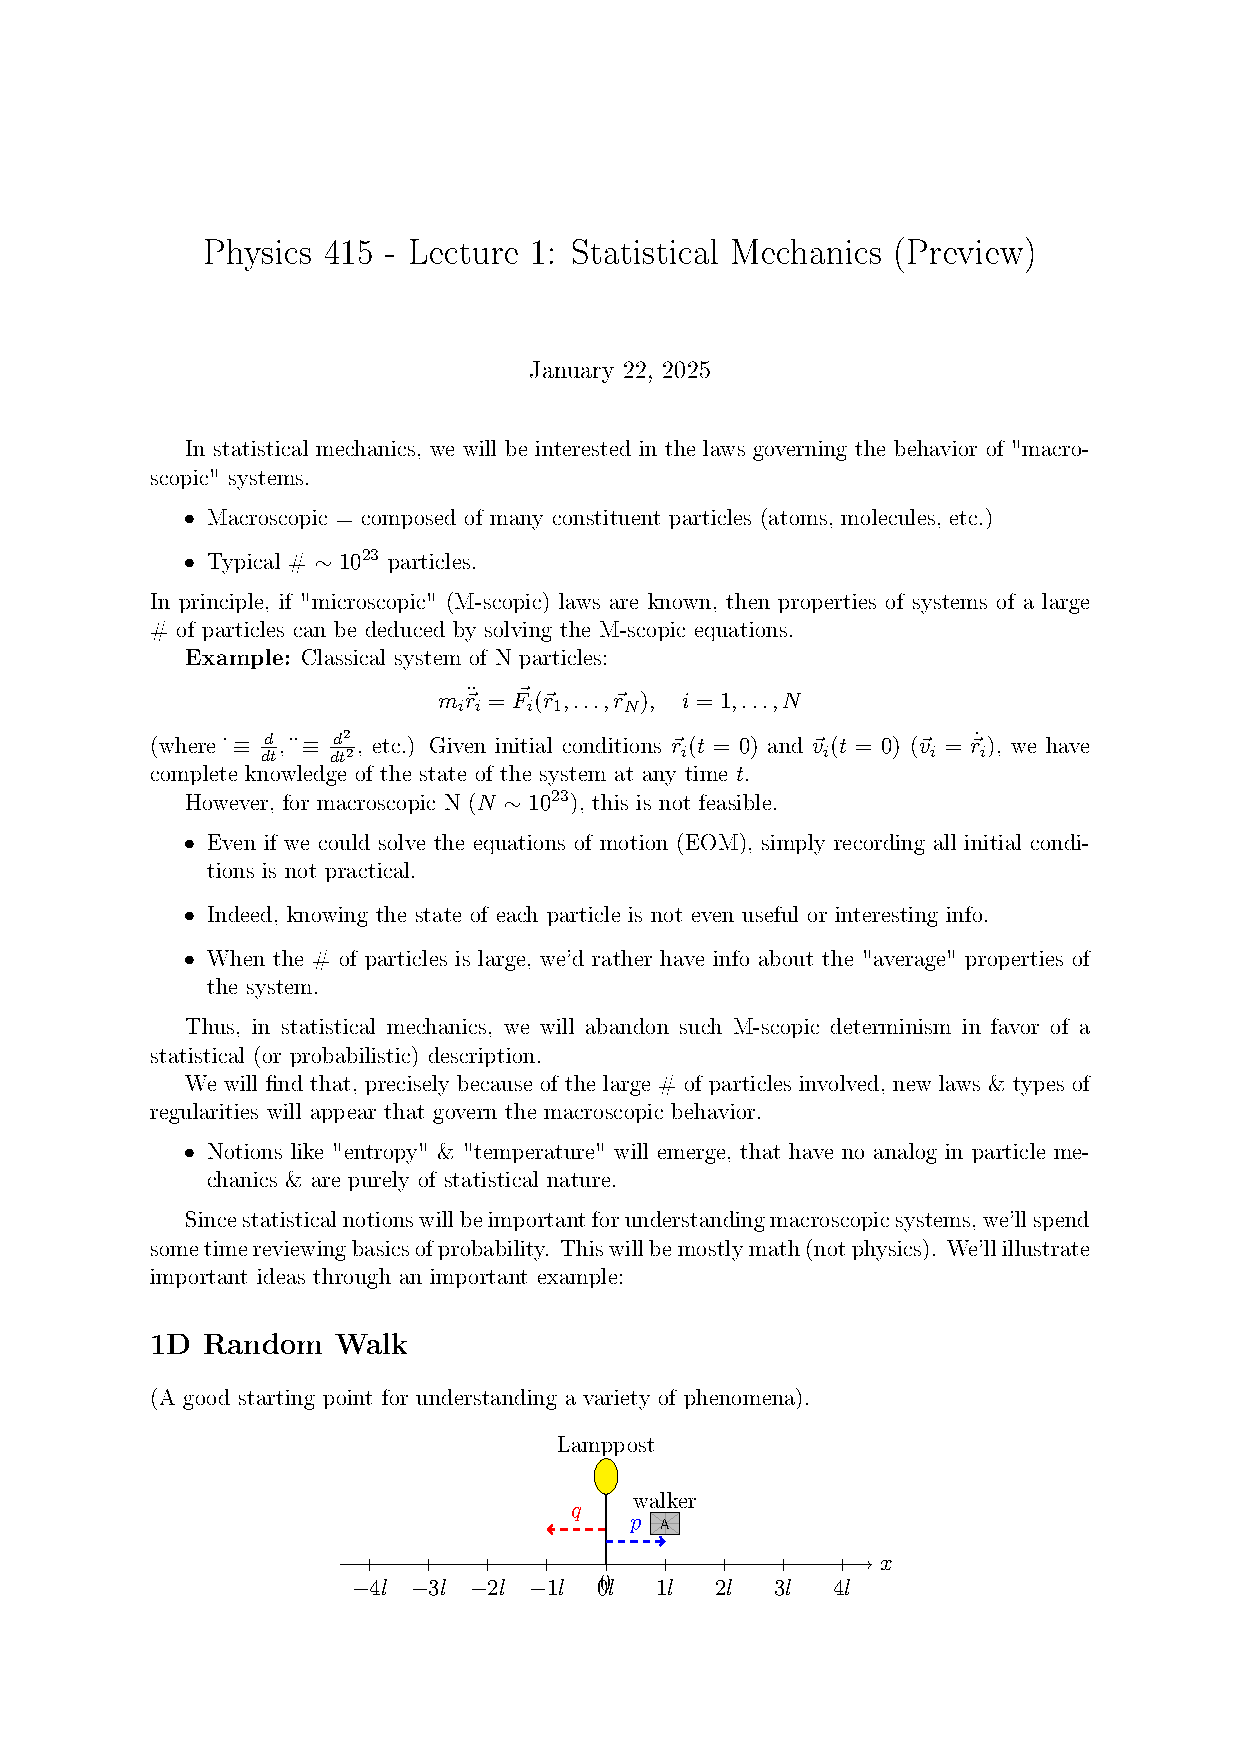
\includepdf[pages=-]{1.pdf}

% --- Include the second PDF ---
\cleardoublepage % Start next included PDF on a right-hand page

% WORKAROUND: Add \phantomsection before \addcontentsline
\phantomsection
\addcontentsline{toc}{chapter}{Lecture 2 (Manual Target)} % Add entry to ToC
% Include 2.pdf WITHOUT linktodoc=true
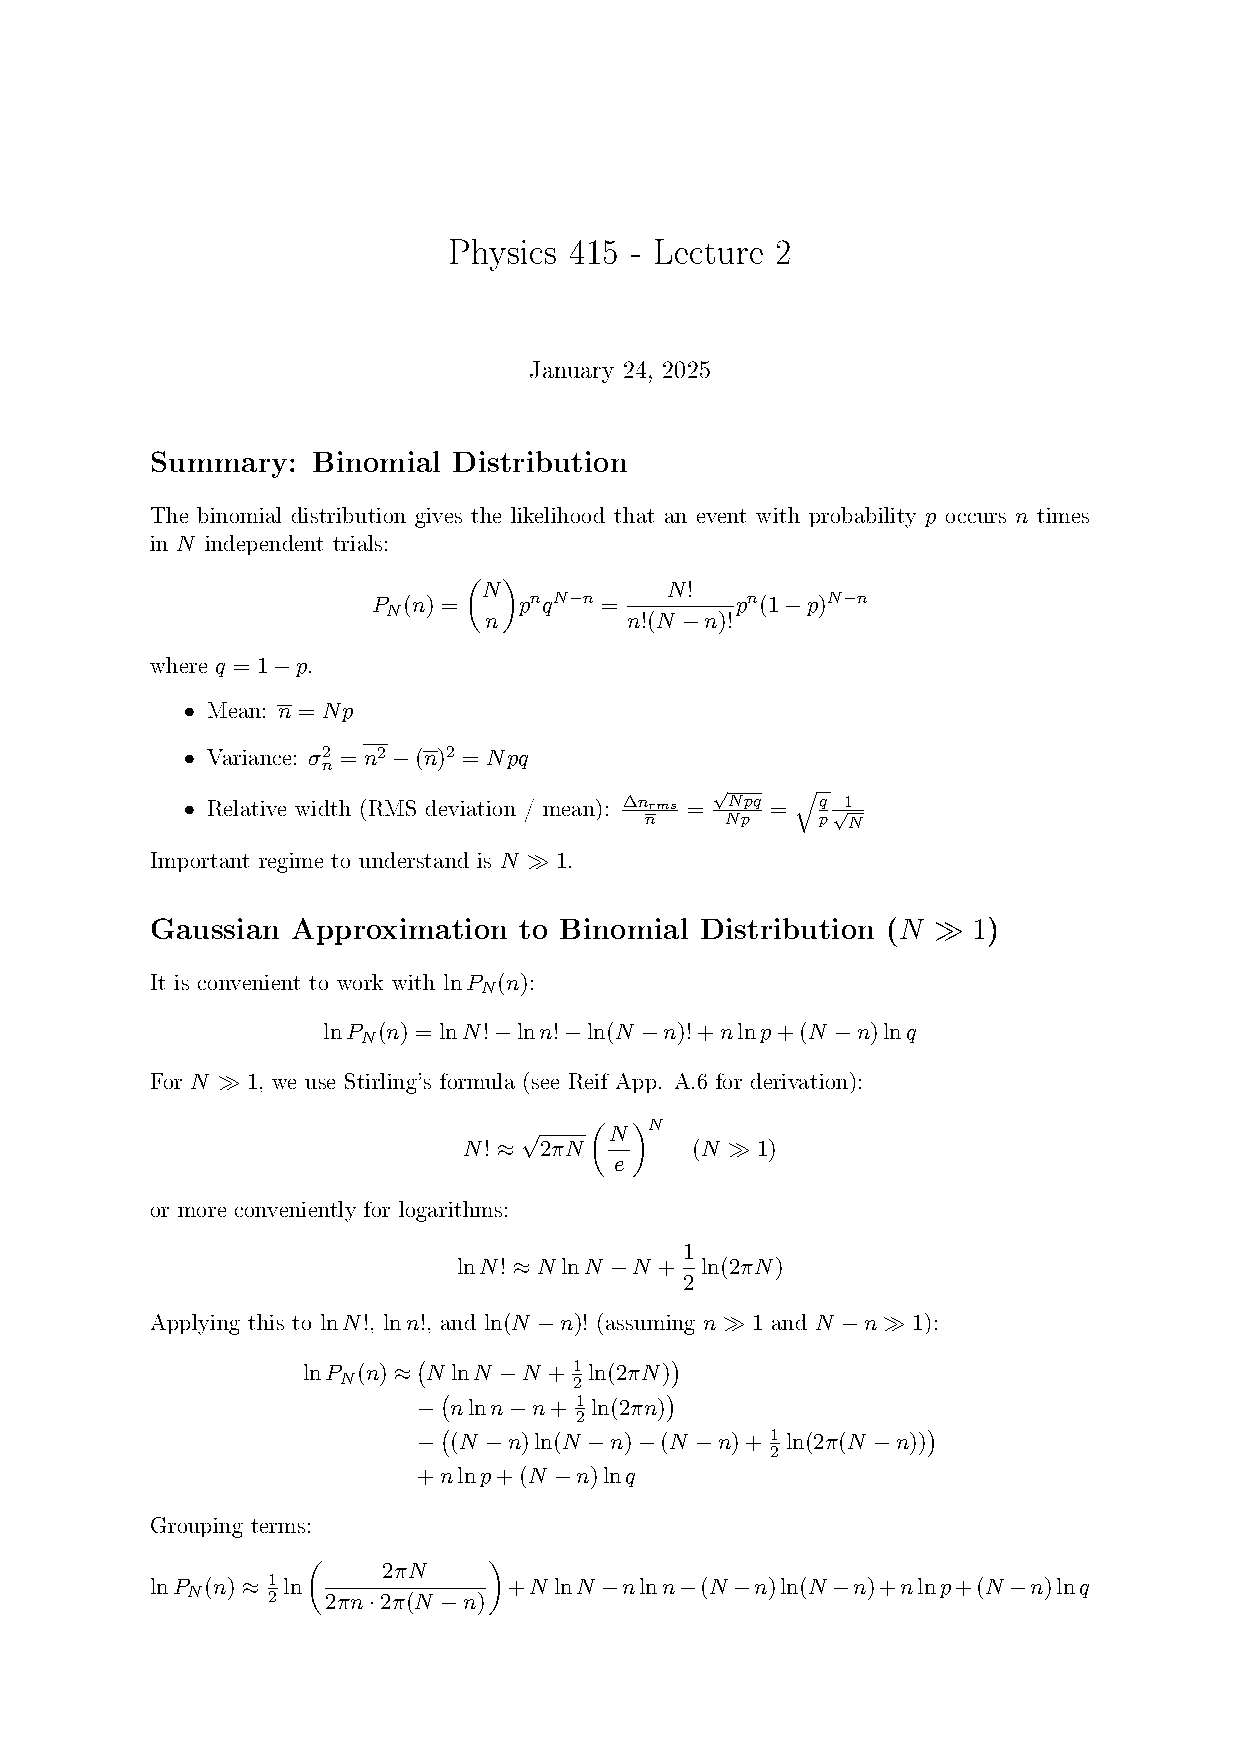
\includepdf[pages=-]{2.pdf}

\end{document}